\section{Constructing contexts and zippers from data types}

The key intuition is that a zipper is a ``focus'' on a subterm of a
term. The data needed to capture this idea is a pair,
\lstinline[language=Scala,mathescape=true]!(T,$\partial$)!, the
subterm itself, and the context in which it occurs. Using types to
guide our intuition we see that the subterm must have the same type as
a term while the type of a context is determined by a calculation that
perfectly matches a version of the derivative one might have learned
in high school calculus -- but applied to data structures.

\subsection{Contexts}

\begin{figure}[tbp]
\begin{center}
{ 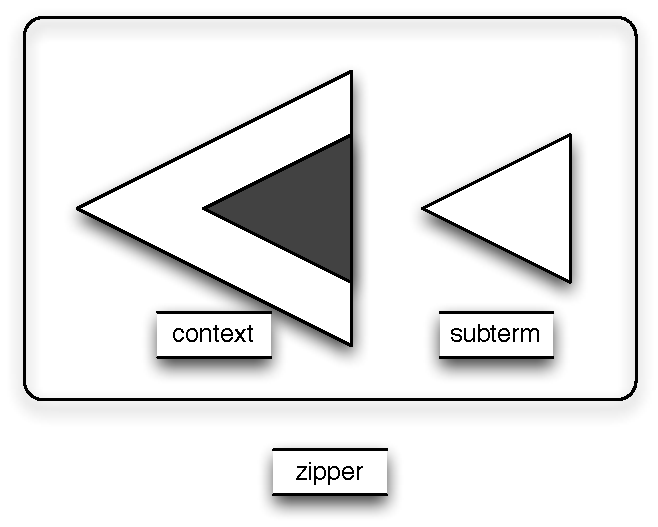
\includegraphics[scale=.65]{/Users/lgm/work/src/projex/biosimilarity/trace/src/main/book/content/figures/ZipperContext1.pdf} }
\caption{ Context and subterm }
\end{center}
\end{figure}

\begin{mathpar}
  \inferrule* {} {\partial Const_A = 0}
  \\
  \inferrule* {} {\partial Id = 0}
  \\
  \inferrule* {} {\partial F + G = \partial F + \partial G}
  \\
  \inferrule* {} {\partial F \times G = F \times \partial G + \partial F \times G}
  \\
  \inferrule* {} {\partial F \circ G = \partial F \circ G \times G}
\end{mathpar}

\begin{figure}[tbp]
\begin{center}
{ 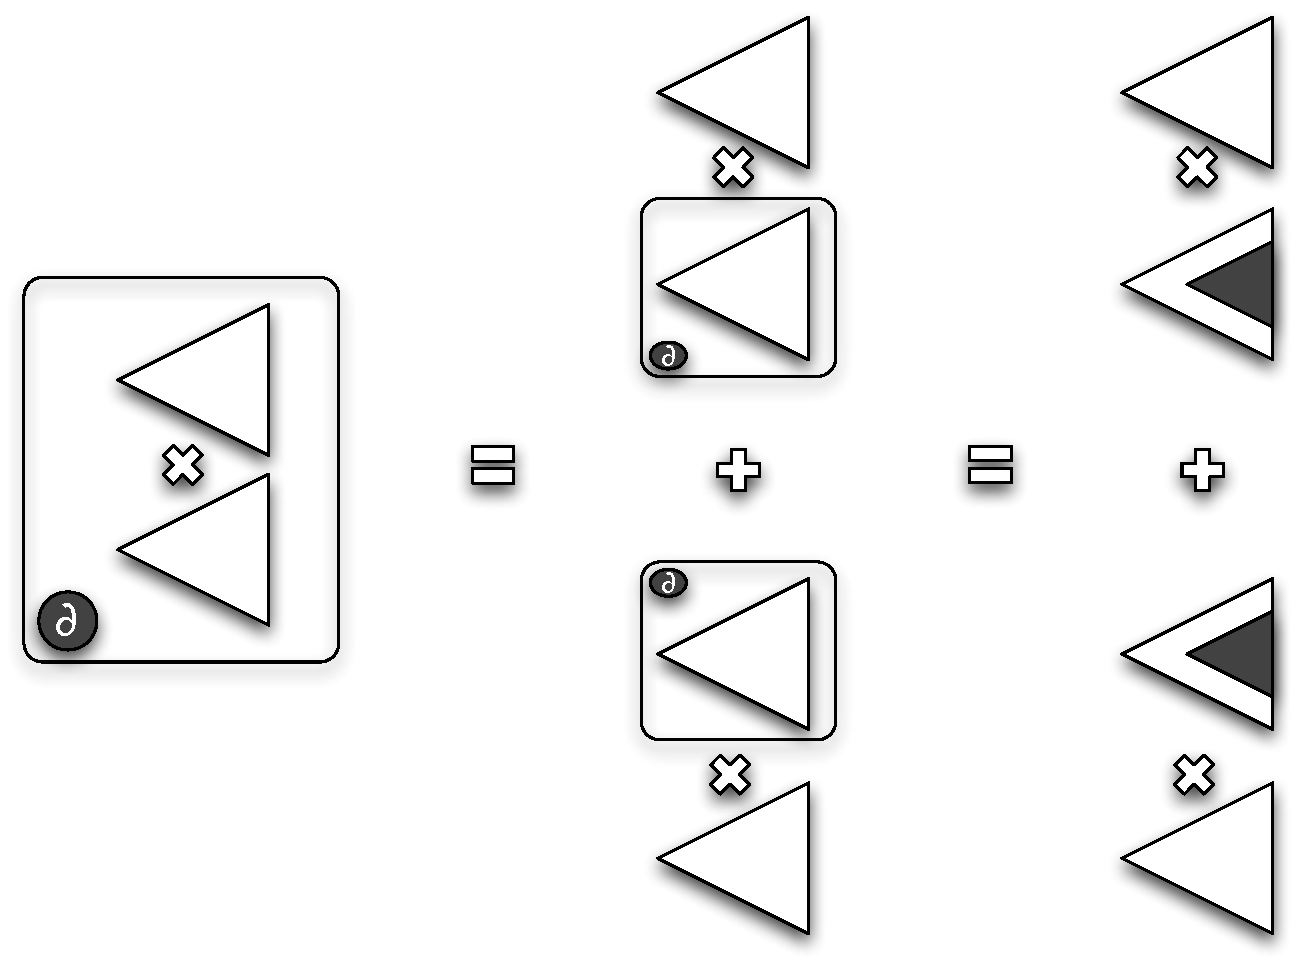
\includegraphics[scale=.75]{/Users/lgm/work/src/projex/biosimilarity/trace/src/main/book/content/figures/Derivative.pdf} }
\caption{ Context and subterm }
\end{center}
\end{figure}

\subsection{Zippers}

\begin{lstlisting}[language=Scala]
  case class Context[Name, NSeq <: NmSeq[Name]](
     override val self : RegularType[Name,NSeq]
  )
  extends RegularType[Name, NSeq] with Proxy {
    override def support = self.support
  }

  trait Contextual[Name, NSeq <: NmSeq[Name]]
  extends Differential[Name,NSeq]  {
    def holePunch( support : NSeq )(
       x : Name, regularType : RegularType[Name,NSeq]
    ) : Context[Name,NSeq] = {
      fresh match {
        case None => throw new Exception( "out of names" )
        case Some( cX ) => {
          val fixRT =
	  RegularFixPt[Name,NSeq](
             (fresh match {
               case None =>
                  throw new Exception( "out of names" )
               case Some( fX ) => fX
             }),
             regularType,
             support
          )
          Context[Name,NSeq](
	     RegularFixPt[Name,NSeq](
                cX,
             RegularSum[Name,NSeq](
                List(
		   RegularUnity[Name,NSeq]( support ),
                   RegularProduct[Name,NSeq](
                      List(
                         RegularFPEnv[Name,NSeq](
                         x,
                         partial( x, regularType ),
                         fixRT,
                         support
		         ),
                         RegularMention[Name,NSeq](
                            cX,
                            support
                         )
		      ),
                      support
                   )
                ),
                support
             ),
             support
           )
        )
      }
    }
  }
}
\end{lstlisting}

\begin{lstlisting}[language=Scala,mathescape=true]
  trait Differential[Name, NSeq <: NmSeq[Name]] 
  extends NmSeqOps[Name,NSeq] {
    def regularNull( supp : NSeq ) : RegularNullity[Name,NSeq]
    def regularUnit( supp : NSeq ) : RegularUnity[Name,NSeq]
    def partial( x : Name, rtype : RegularType[Name, NSeq] )
    : RegularType[Name, NSeq] = {
      rtype match {
        case RegularMention( y, supp ) => {
          if ( x == y ) {
            regularUnit( supp )
          }
          else {
            regularNull( supp )
          }
        }
        case RegularNullity( supp ) => regularNull( supp )
        case RegularUnity( supp ) => regularNull( supp )
        case RegularSum( s, supp ) => {
          RegularSum(
	     s.map(
               {
                 ( rt : RegularType[Name,NSeq]) => {
                   partial( x, rt )
                 }
               }
             ),
             supp
          )
        }
        case RegularProduct( s, supp ) => {
          val right = s.dropRight( 1 )
          RegularSum[Name,NSeq](
	     List(
                RegularProduct[Name,NSeq](
                   List(
                      partial( x, s( 0 ) ),
                      RegularProduct[Name,NSeq](
                         right,
                         supp
                      )
                   ),
                   supp
                ),
                RegularProduct[Name,NSeq](
                   List(
                      s( 0 ),
                      partial(
                         x,
                         RegularProduct[Name,NSeq]( right, supp )
                      )
                   ),
                   supp
                )
	     ),
             supp
	  )
        }
        case RegularFixPt( v, e, supp ) => {
          val z = fresh match {
            case None => throw new Exception( "out of names" )
            case Some( fn ) => fn
          }
          RegularSum[Name,NSeq](
	     List( 
                RegularFixPt(
                   z, 
                   partial(
		      x,
                      RegularWeakening(
                         z,
                         RegularFPEnv( v, e, rtype, supp ),
                         supp
                      )
                   ),
                   supp
                ),
                RegularProduct(
                   List(
                      partial(
                         v,
                         RegularFPEnv(
                            v,
                            e,
                            rtype,
                            supp
		         )
                      ),
                      RegularMention( z, supp )
                   ),
                   supp
                )
             ),
             supp
	   )
         }
         case RegularFPEnv( v, e, s, supp ) => {
           RegularSum(
              List(
                 RegularFPEnv(
                    v,
                    partial( x, e ),
                    s,
                    supp
                 ),
                 // BUGBUG -- lgm -- have i got the association correct
                 RegularProduct(
                    List(
                       RegularFPEnv(
                          v,
                          partial( v, e ),
                          s,
                          supp
                       ),
                       partial( x, s )
                    ),
                    supp
                 )
              ),
              supp
           )
         }
         case RegularWeakening( v, e, supp ) => {
           if ( x == v ) {
             regularNull( supp )
           }
           else {
             RegularWeakening( v, partial( x, e ), supp )
           }
         }
       }
     }
   }
\end{lstlisting}